\chapter{Diffraction}
The spreading out of wave when it passes through a narrow opening is usually referred to as diffraction and the intensity distribution on the screen is known as the diffraction pattern.The spreading out decreases with decrease in wavelength .Indeed since the light wavelength are very small the effect due to diffraction are not readily observed.\\
Difference between the phenomena of interferene and diffraction is that ,interfernece corresponds to the situation when we consider the superposition of waves coming out from a numnber of point sources and the diffraction corresponds to the situation when we consider waves coming out from a area source like circular, or rectangular aperture or even a large munber of rectangular apertures(grating).\\
The diffraction phenomena are further classified in to two\\
(a) Fresnal diffraction \\
(b)Fraunhofer diffraction.\\
In the Fresnal class of diffraction the sources of light and the screen are in general at a finite distance from the diffracting apperture.In fraunhofer class of diffraction the source and the screen are at definite distance from the aperture.This is easily achieved by placing two convex lens with source at the focal plane of one covex lens and placing screen on the focal plane of other convex lens.\\
\section{Fraunhofer diffraction}
\subsection{Single slit diffraction pattern}
\begin{figure}[H]
	\centering
	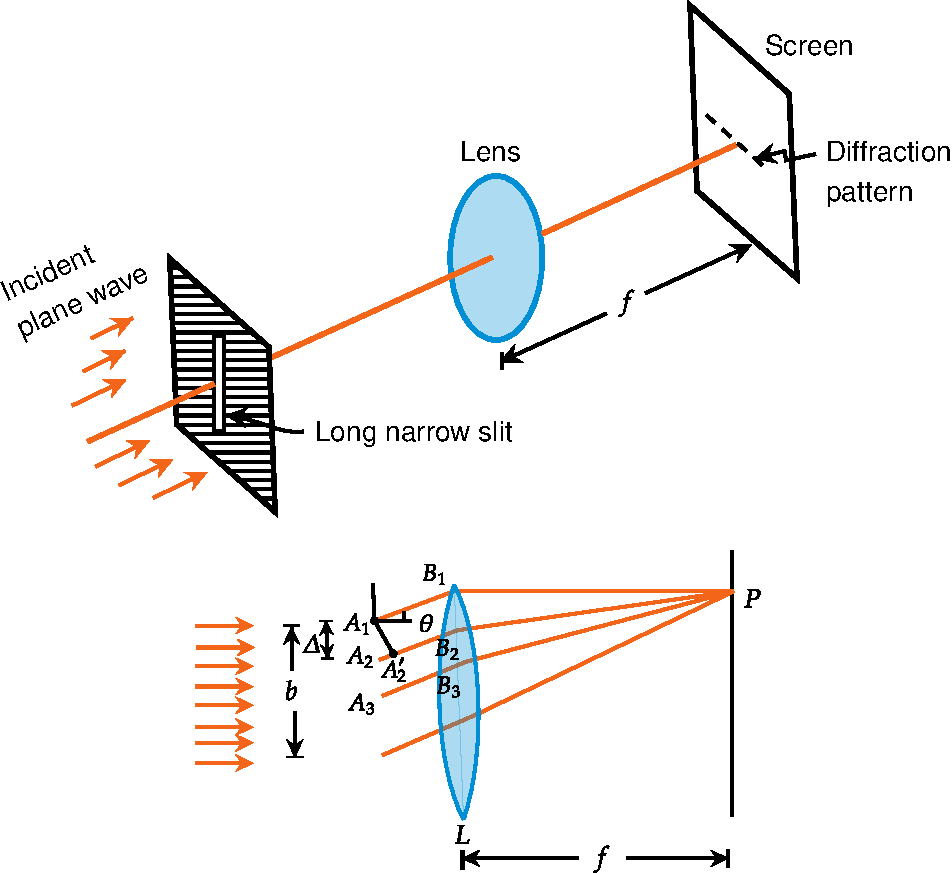
\includegraphics[height=8cm,width=10cm]{diagram-20211220-crop}
	\caption{}
	\label{}
\end{figure}
A plane wave is assumed to fall normally on the slit of width b and we wish to calculate the intensity distribution on the focal plane of the lens L.Now divide the slit in to number of point sources $A_1,A_2,A_3,...$ Let the seperation between two sources to be $\Delta$.Suppose there are n point sources then we can write\\
$$b=(n-1)\lambda$$
We have to find the resultant field at p due to all n sources.The optical path difference between the disturbance from the point $A_1$ and $A_2$ will be $A_2A_2^{\prime}$(see figure)\\
$$A_2A_2^{\prime}=\Delta \sin \theta$$
Where $\theta$ angle between the diffracted ray and the normal to the slit.\\
Then phase difference will be \\
$$\phi=\frac{2\pi}{\lambda}\Delta \sin \theta$$
The field at P due to $A_1$ is\\
$$E_1=a \cos\omega t$$
The field at P due to $A_2$ is\\
$$E_1=a (\cos\omega t-\phi)$$\\
The total field at P due to the points $A_1,A_2,A_3,...$  is \\
$$E=a\left[ \cos\omega t+\cos(\omega t-\phi)+...+\cos(\omega t-(n-1))\phi\right] $$
But$$\left[ \cos\omega t+\cos(\omega t-\phi)+...+\cos(\omega t-(n-1))\phi\right]=\frac{\sin n\phi/2}{\sin \phi/2}\cos\left[ \omega t-\frac{1}{2}(n-1)\phi\right] $$
Thus \\
$$E=E_0\cos\left[ \omega t-\frac{1}{2}(n-1)\phi\right] $$
Where $E_{\theta}$ is the amplitude of the resultant field.\\
$$E_{\theta}=a\frac{\sin n \phi/2}{\sin \phi/2}$$
In the limit of $n\rightarrow \infty$ \quad \quad $n\Delta \rightarrow$ to b\\
Then \\
$$\frac{n\phi}{2}=\frac{\pi}{\lambda} n\Delta \sin \theta \rightarrow \frac{\pi}{\lambda}b \sin \theta$$
Further $$\phi=\frac{2\pi}{\lambda} \Delta \sin \theta=\frac{2\pi}{\lambda}\frac{b\sin \theta }{n}$$
THen $$E_{\theta}=na\frac{\frac{\sin \pi b \sin \theta}{\lambda}}{\frac{\pi b \sin \theta}{\lambda}}$$
$$=\frac{\sin \beta}{\beta}$$
Where $A=na$ and $\beta=\frac{\pi b \sin \theta}{\lambda}$
$$E=A\frac{ \sin \beta}{\beta} \cos(\omega t-\beta)$$
The corresponding intensity distribution is given by
$$I=I_0\frac{\sin^2\beta}{\beta^2}$$
Where $I_0$ represents intensity at $\theta=0$\\
\begin{note}
(i)The variation intensity $\beta$ is shown in the figure.
\begin{figure}[H]
	\centering
	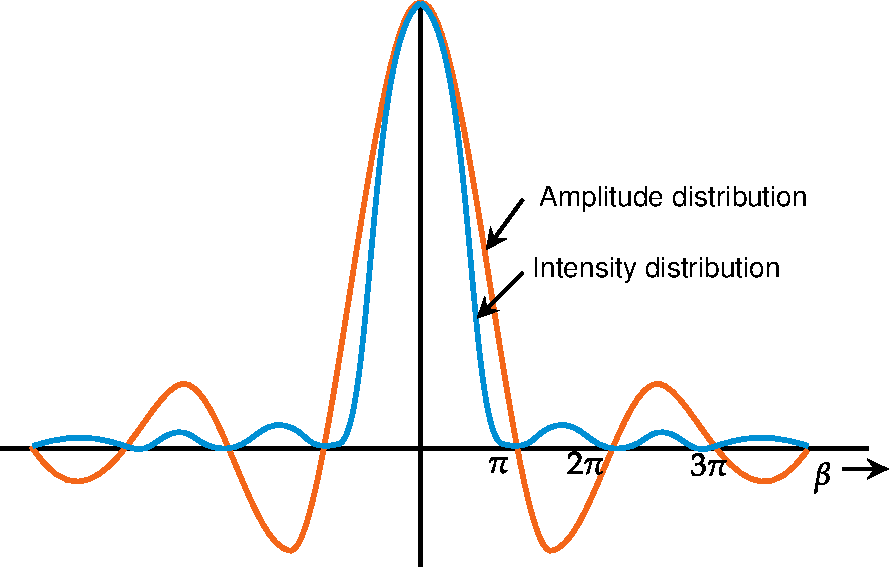
\includegraphics[height=5cm,width=8cm]{diagram-20211220(1)-crop}
	\caption{}
	\label{}
\end{figure}
(ii)The width of the central maxima is $\left( \frac{2\lambda D}{b}\right)$ \\
And the angular width of central maxima is $\left( \frac{2\lambda}{b}\right)$ 	
\end{note}
\begin{exercise}
	A plane wave of wavelength 6250$A^{\circ}$ is incident normally on a slit of width $2\times 10^{-2}$cm.The width of the principal maximum on a screen distant 50cm will be?
\end{exercise}
\begin{answer}
Width of the central maximum\\
$$=\frac{2\lambda D}{a}=\frac{2\times 6250 \times10^{-10}\times 0.5}{2\times 10^{-4}}$$
$$=3125\times 10^{-3}cm$$
\end{answer}
\subsubsection{Position of maxima and minina}
\paragraph{minima}
Intensity is zero when\\
$$\beta=m\pi,m\neq0$$
$$\implies b\sin \theta =m\lambda;m=\pm 1,\pm 2,\pm3,....$$
\paragraph{maxima} 
In order to determine the position of maxima we differentiate equation$$I=I_0\frac{\sin^2\beta}{\beta^2}$$ with respect to $\beta$ and set it equals to zero.\\Thus
$$\frac{dI}{d\beta}=I_0\left[ \frac{2\sin\beta \cos\beta}{\beta^2}-\frac{2\sin^2 \beta}{\beta^3}\right] =0$$
$$\sin\beta\left[ \beta-\tan \beta\right] =0$$
The condition $\sin \beta=0$ or $\beta=m\pi$ corresponds to minima.\\
The condition for maxima are the roots of the equation\\
$$\beta=\tan \beta$$
$\beta=0$ corresponds to central maxima.\\
The position of other maxima will get from the the metting point of $y=\beta$ and $y=\tan \beta$ of the figure shown bellow.
\begin{figure}[H]
	\centering
	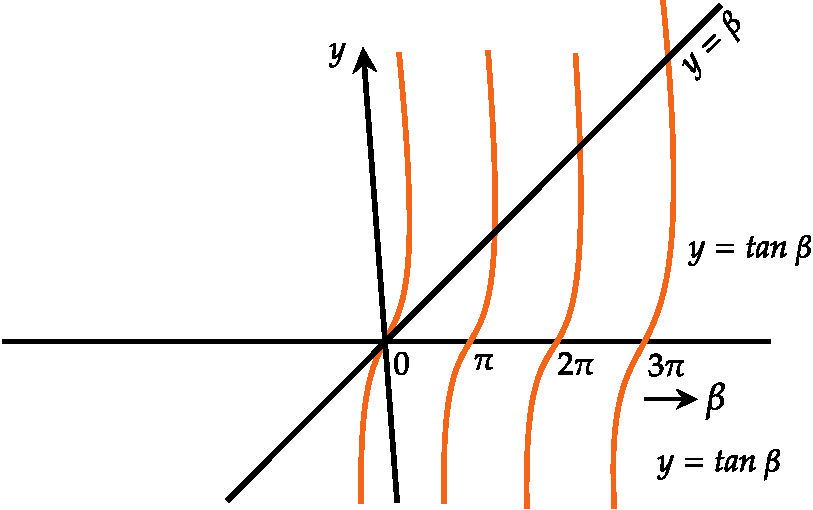
\includegraphics[height=5cm,width=8cm]{diagram-20211220(2)-crop}
	\caption{}
	\label{}
\end{figure}
For first maxima $\beta=1.43\pi$\\
For second maxima $\beta=2.46\pi$
\subsection{Two slit diffraction pattern}
\begin{figure}[H]
	\centering
	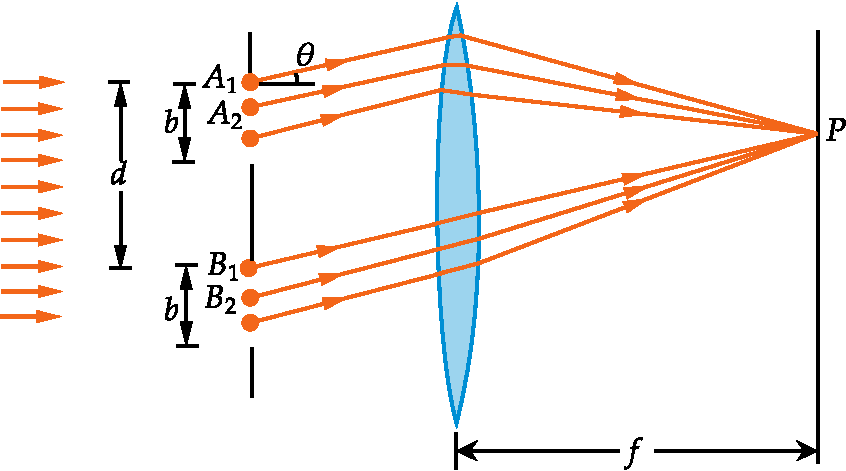
\includegraphics[height=5cm,width=8cm]{diagram-20211221(1)-crop}
	\caption{}
	\label{}
\end{figure}
Now we consider two parallel slits (each of width b) seperated by a distance d.We found find that the resultant intensity is the product of the single slit diffraction pattern and the interference pattern produced by two point sources sepserated by a distance d.\\
The two slits are divided into equally spaced point sources.$A_1,A_2,A_3,...$ as the first slit and $B_1,B_2,B_3,....$ as the second slit.\\
The electric field at the point P due to the first slit is \\
$$E_1=A \frac{\sin \beta}{\beta} \cos (\omega t-\beta)$$
similarly the second will produce a field\\
$$E_2=A \frac{\sin \beta}{\beta} \cos (\omega t-\beta-\upPhi)$$
Where $$\upPhi=\frac{2\pi}{\lambda}d \sin \theta$$
Where $\upPhi$ is the phase difference between the disturbance from the two slits.\\
$$E=E_1+E_2$$
$$=A \frac{\sin \beta}{\beta}\left[ \cos(\omega t-\beta)-\cos(\omega t-\beta -\upPhi)\right] $$
Which represents the interference of two waves ,each of an amplitude A$\frac{\sin \beta}{\beta}$ and differing in phase by $\upPhi$.It can be rewritten as \\
$$E=A \frac{sin\beta}{\beta} \cos\gamma \cos\left( \omega t-\frac{\beta}{2}-\frac{\upPhi}{2}\right) $$
Where $$\gamma=\frac{\upPhi}{2}=\frac{\pi}{\lambda}d\sin\theta$$
Intensity distribution will be of the form,
$$I_0=4I_0\frac{\sin^2\beta}{\beta^2}\cos^2\gamma$$
The intensity distribution is the product of two terms,the first term ($\frac{\sin^2\beta}{\beta^2}$)represents the diffraction pattern produced by a single slit of width b and and the second term represents ($\cos^2\gamma$) represents the interfernce pattern produced by two point sources seperated by a distance d.\\
\paragraph{Positions of maxima and minima}
\begin{figure}[H]
	\centering
	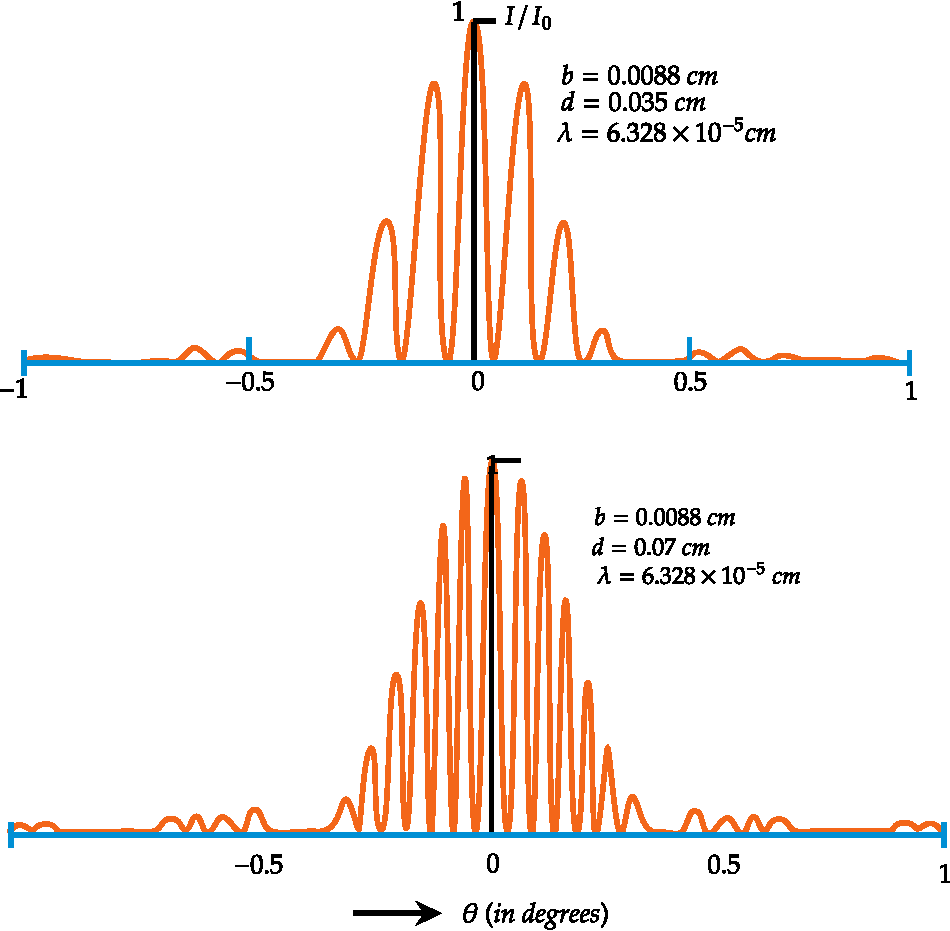
\includegraphics[height=8cm,width=16cm]{diagram-20211223-crop(1)}
	\caption{}
	\label{}
\end{figure}
\paragraph{Minima}
The equation tell us that the intensity is zero whenever,
$$\beta=\pi,2\pi,3\pi,...$$
or when $$\gamma=\frac{\pi}{2},\frac{3\pi}{2},\frac{5\pi}{2},....$$
Now the conditions become \\
$$b\sin \theta=m\lambda;\quad \quad (m=1,2,3,...)$$
$$d\sin \theta=\left( n+\frac{1}{2}\right) ; \quad \quad (n=1,2,3,....)$$
\paragraph{maxima}
$$\gamma=0,\pi,2\pi....$$
or when $$d\sin \theta=0,\lambda,2\lambda,2\lambda,2\lambda,....$$
But a maxima will not occur when at all if $\theta$ corresponds to a diffraction minimum.ie if $b\sin \theta=\lambda,2\lambda,3\lambda,....$.These are usually referred to as missing orders.
\subsection{N slit fraunhofer diffraction pattern}
\begin{figure}[H]
	\centering
	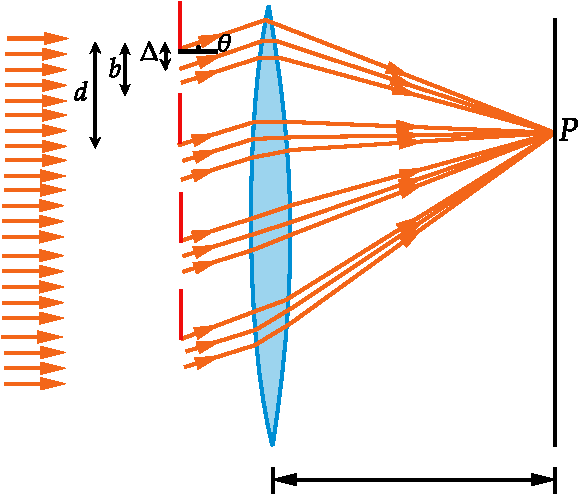
\includegraphics[height=5cm,width=8cm]{diagram-20211221(2)-crop}
	\caption{}
	\label{}
\end{figure}
We next consider the diffraction pattern produced by $N$ parallel  slits, each of width $b$; the distance between two consecutive slits is assumed to be $d$.

As before, we assume that each slit consists of $n$ equally spaced point sources with spacing $\Delta$  Thus the field at an arbitrary point $P$ will essentially be a sum of $N$ terms:
$$\begin{aligned}
	E=& A \frac{\sin \beta}{\beta} \cos (\omega t-\beta)+A \frac{\sin \beta}{\beta} \cos \left(\omega t-\beta-\Phi_{1}\right) \\
	&+\ldots+A \frac{\sin \beta}{\beta} \cos \left(\omega t-\beta-(N-1) \Phi_{1}\right)
\end{aligned}$$
where the first term represents the amplitude produced by the first slit, the second term by the second slit, etc.Rewritting the equation we will get
$$\begin{aligned}
	E=& \frac{A \sin \beta}{\beta}\left[\cos (\omega t-\beta)+\cos \left(\omega t-\beta+\Phi_{1}\right)\right.\\
	&\left.+\ldots+\cos \left(\omega t-\beta-(N-1) \Phi_{1}\right)\right] \\
	=& \frac{A \sin \beta}{\beta} \frac{\sin N \gamma}{\sin \gamma} \cos \left[\omega t-\beta-\frac{1}{2}(N-1) \Phi_{1}\right]
\end{aligned}$$
where
$$
\gamma=\frac{\Phi_{1}}{2}=\frac{\pi}{\lambda} d \sin \theta
$$
The corresponding intensity distribution will be
$$
I=I_{0} \frac{\sin ^{2} \beta}{\beta^{2}} \frac{\sin ^{2} N \gamma}{\sin ^{2} \gamma}
$$
where $I_{0} \sin ^{2} \beta / \beta^{2}$ represents the intensity distribution pro duced by a single slit.the intensity distribution is the product of two terms;The first term $\left( \frac{\sin^2\beta}{\beta^2}\right)$  diffraction pattern produced by a single slit and the second term represents $\left( \frac{\sin^2N \gamma}{\sin^2 \gamma}\right) $represents the interference pattern produced by N equally spaced point sources.\\
When N icreases the the sharpness of the peak also increases.\\
The function vanishes between two peaks when 
$$\gamma=\frac{p\pi}{N};p=\pm1,\pm2,\pm3,... \text{but} p\neq0,\pm N,\pm2N$$
Which are reffered to as secondary minima.\\
\begin{figure}[H]
	\centering
	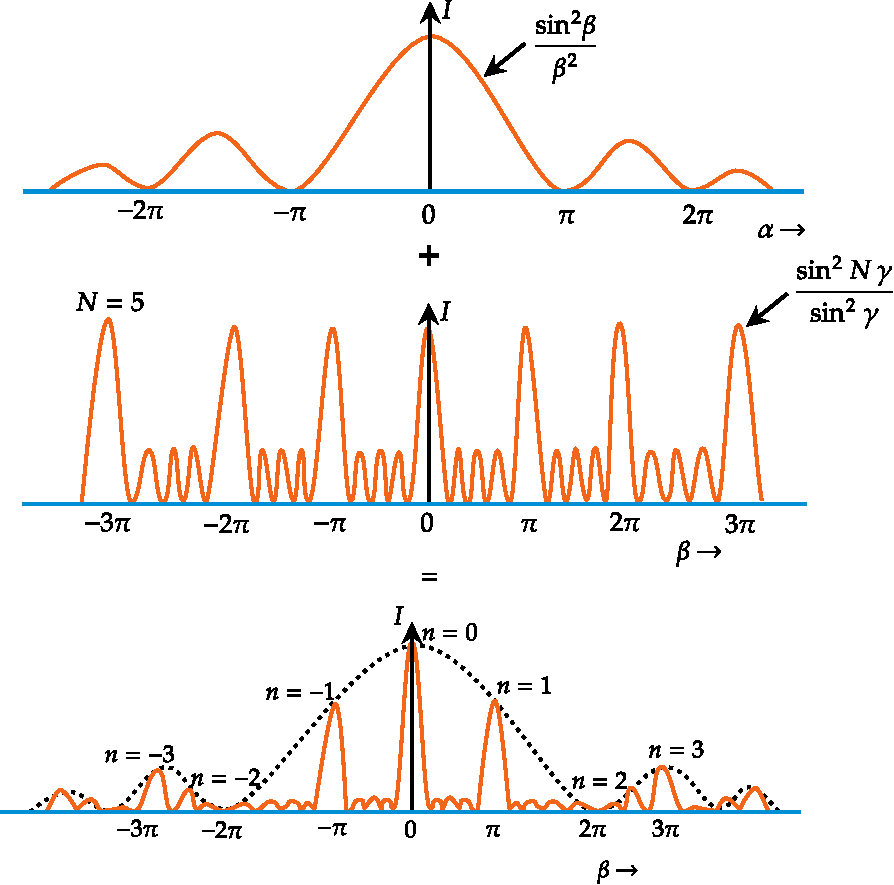
\includegraphics[height=10cm,width=15cm]{diagram-20211223(19)-crop}
	\caption{}
	\label{}
\end{figure}
\textbf{Positions of maxima  and minima}\\
\textbf{maxima}\\
When the value of N is very large one obtain intense maxima at $\gamma=m\pi$ when$$d\sin \theta=m\lambda  (m\lambda=0,1,2,3....)$$
At $\gamma=m\lambda$ \\
$$\underset{\gamma \rightarrow m \pi}{L t} \frac{\sin N \gamma}{\sin \gamma}=\underset{\gamma \rightarrow m \pi}{L t} \frac{N \cos N \gamma}{\cos \gamma}=\pm N$$
thus, the resultant amplitude and the corresponding intensity distributions are given by
$$
E=N \frac{A \sin \beta}{\beta}
$$
$$
I=N^{2} I_{0} \frac{\sin ^{2} \beta}{\beta^{2}}
$$
where
$$
\beta=\frac{\pi b \sin \theta}{\lambda}=\frac{\pi b}{\lambda} \frac{m \lambda}{d}=\frac{\pi b m}{d}
$$
Such maxima are called principal maxima.\\
\textbf{Minima}\\
The minima will obtain when \\
$$b\sin\theta=n\lambda,n=1,2,3,...$$
Gives us the minima correspondings to the single slit diffraction pattern.
$$N\gamma=p\pi,p=N,2N,....$$ The angle of diffraction of the above equation is \\
$$d\sin \theta=\frac{\lambda}{N},\frac{2\lambda}{N},....,\frac{(N-1)\lambda}{N},\frac{(N+1)\lambda}{N},\frac{(N+2)\lambda}{N},.....\frac{(2n-1)\lambda}{N},\frac{(2N+1)\lambda}{N},\frac{(2N+2)\lambda}{N},....$$
Thus we have two principal maxima we have (N-1) Minimas.Betweeen two consecutive minima the intensity has to have a maximum,these maxima are known as secondary maxima.\\
\begin{note}
	\begin{enumerate}
	\item A particular maxima may be absent if it corresponds to the angle which also determines the minima of the sigle slit diffraction pattern.This will happen when 
	$$d\sin \theta =m\lambda$$
	$$b\sin\theta=\lambda,2\lambda,3\lambda...$$
	are satisfied simultaneously and usually referredto as a missing order.\\
	\item Diffraction minimas will be very small if N is very small.
		\end{enumerate}
\end{note}
\textbf{Width of the principal maxima}
The $m^{(th)}$ order principal maxima occurs at \\
$$d\sin \theta_{m}=m\lambda,m=0,1,2,3,....$$
The minima occures at the angle given by 
$$d\sin\theta=\frac{\lambda}{N},\frac{2\lambda}{N},...$$
If $\theta_m+\Delta \theta_{1m}$ and $\theta_m-\Delta \theta_{2m}$ represents the angle of diffraction corresponding to the first maximum on either side of the principal maximum, then $\frac{1}{2}(\Delta \theta_m+\Delta \theta_{2m})$ is known as the angular width of the mth order principal maximum.For large value of N $\Delta\theta_{1m}=\Delta\theta_{2m}$ which we write as $\Delta \theta_m$\\
clearly $$d\sin(\theta_m\pm\Delta\theta_m)=m\lambda\pm\frac{\lambda}{N}$$
But\\
$$\sin(\theta_m\pm\Delta \theta_m)=\sin\theta_m \cos \Delta\theta_{m}\pm\cos \theta_m\sin\Delta \theta_m$$
$$=\sin\theta_{m}\pm\Delta \theta_{m}\cos\theta_{m}$$
$$\Delta\theta_{m}=\frac{\lambda}{Nd\cos \theta_m}$$
Which shows that the principal maximum becomes sharper as N increases.
\subsection{The diffraction grating}
 An arrangement which essentially consisit of a large number of equidistant slits is known as diffraction grating.The corresponding diffraction pattern is known as diffraction spectra.For a narrow principal maxima a large number of N is required.\\
 \textbf{Properties of grating spectra}
 \begin{enumerate}
 	\item The positions of principal maxima are given by \\
 	$$d\sin \theta=m\lambda; \quad m=0,1,2,3,....$$
 	The equation is known as grating equation.
 	\item The zeroth order principal maximaum ($\theta
 	=0$) is known as central maxima. And it will have the colour of the source used.White if polychromatic source is used.
 	\item If $m\neq0$ the angle of diffraction are different for different wavelength and therefore and various spectral component will appear at different positions.Thus  measuring the angle of diffraction one can determine the wavelength.
 	\item Intensity is maximum for zeroth order spectra(Where there is no dispersion) and intensity decreases when m increases.
 	\item $$d\sin \theta=m\lambda$$ differentiating with respect to $\lambda$ we will get\\
 	$$\frac{\Delta \theta}{\Delta \lambda}=\frac{m}{d \cos \theta}$$
 	when $\theta$ is very small $\cos\theta=1$ and for a given m \\
 	$\frac{\Delta \theta}{\Delta \lambda}$ is a constant.Such a spectrum is konwn as normal spectrum.
 	\item $\Delta \theta$ is inversily proportional to d,Therefore the smaller the grating element the larger will be the angular dispersion.
 	\item If we use point sources on a focal plane of a $L_1$ and we will get line spectrum on the focal plane the lens $L_2$ .If we use slit we will get band spectrum.
 	Where $L_1$ is used to focus the light coming from the sources to grating.$L_2$ is the lens used to focus light from grating to the screen.
 \end{enumerate}
\subsection{Resolving power of a grating}
The resolving power is the power of distiquishing two nearby spectral lines and is defined by the equation :
$$R=\frac{\lambda}{\Delta \lambda}$$
Where $\Delta \lambda$ is the seperation of two wavelength which the grating can just resolve;The smaller the value of $\Delta \lambda$, the larger the resolving power.\\
\begin{figure}[H]
	\centering
	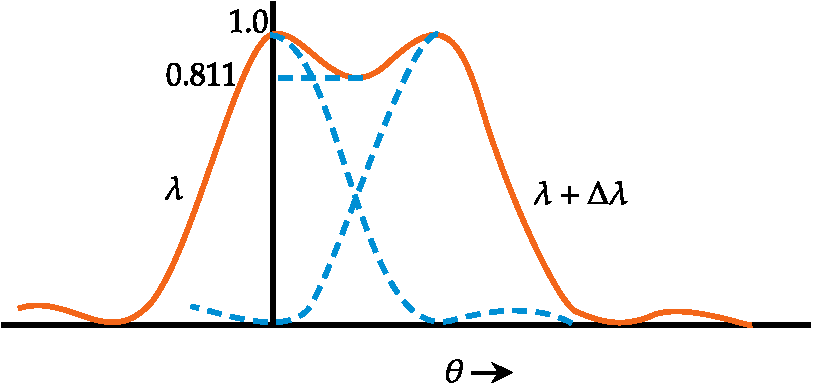
\includegraphics[height=5cm,width=8cm]{diagram-20211221(6)-crop}
	\caption{}
	\label{}
\end{figure}
The Rayleigh criterion can be used to define the limit of resolution. According to this criterion, if the principal maximum corresponding to the wavelength $\lambda$ $+\Delta \lambda$ falls on the first minimum (on the either side of the principal maximum) of the wavelength $\lambda$, then the two wavelengths $\lambda$ and $\lambda+\Delta \lambda$ are said to be just resolved  If this common diffraction angle is represented by $\theta$ and if we are looking at the $m$ th order spectrum, then the two wavelengths $\lambda$ and $\lambda+\Delta \lambda$ will be just resolved if the following two equations are simultaneously satisfied:
$$d \sin \theta=m(\lambda+\Delta \lambda)$$
$$d \sin \theta=m \lambda+\frac{\lambda}{N}$$
$$
R=\frac{\lambda}{\Delta \lambda}=m N
$$
Resolving power depends on the total number of lines in the grating (N).And also proportional to the order of the spectrum.
\begin{exercise}
	When a gaseous elements is raised to very high temperature,the atom emit radiation having discrete wavelength.The two components in the atomic spectrum have wavelength of $5890A^{\circ}$ and $5896A^{\circ}$\\
	(a) what resolving power must a grating have if these wavelength are to be distiguished?\\
	(b)To resolve these lines in the second order spectrum how many slit of the grating must be illuminated?
\end{exercise}
\begin{answer}
(a)Resolving power is 
$$R=\frac{\lambda}{d\lambda}$$
Where $\lambda=\frac{\lambda+\lambda}{2}=\frac{5890+5896}{2}=5893$\\
$\delta \lambda=5896-5890=6A^{\circ}$\\
$R=\frac{5893}{6}=982$\\
(b)$R=mN$\\
$$N=\frac{R}{n}	=\frac{982}{2}=491$$ slits
\end{answer}
\newpage
\begin{abox}
	Previous year solutions
	\end{abox}
\begin{enumerate}
\begin{minipage}{\textwidth}
	\item A monochromatic plane wave (wavelength $=600 \mathrm{~nm}) E_{0} \exp [i(k z-\omega t)]$ is incident normally on a diffraction grating giving rise to a plane wave $E_{1} \exp \left[i\left(\vec{k}_{1} \cdot \vec{r}-\omega t\right)\right]$ in the first order of diffraction. Here $E_{1}<E_{0}$ and $\vec{k}_{1}=\mid \vec{k}_{1}\left[\frac{1}{2} \hat{x}+\frac{\sqrt{3}}{2} \hat{z}\right] .$ The period (in $\mu m$ ) of the diffraction grating is (upto one decimal place)
	\exyear{GATE 2015}
\end{minipage}
\begin{answer}
	\begin{figure}[H]
		\centering
		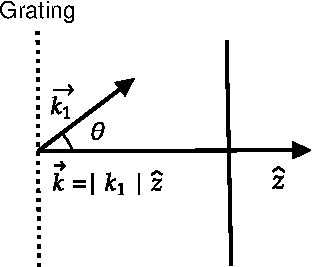
\includegraphics[height=4cm,width=6cm]{pic1-crop}
	\end{figure}
 $d \sin \theta=n \lambda \Rightarrow d=\frac{\lambda}{\sin \theta} \quad \because n=1$
	$$
	\begin{aligned}
	&\text { and } \vec{k}_{1}=\left|\vec{k}_{1}\right|\left[\frac{1}{2} \hat{x}+\frac{\sqrt{3}}{2} \hat{z}\right] \\
	&\Rightarrow \sin \theta=\frac{\vec{k} \times \vec{k}_{1}}{\left|\vec{k}_{1}\right||\vec{k}|}=\frac{\hat{z} \times\left(\frac{1}{2} \hat{x}+\frac{\sqrt{3}}{2} \hat{z}\right)}{\sqrt{\frac{1}{4}+\frac{3}{4}} \times \sqrt{\frac{1}{4}+\frac{3}{4}}}=\frac{1}{2} \Rightarrow \theta=30^{\circ} \\
	&\Rightarrow d=\frac{600}{\sin 30} n m=1200 \mathrm{~nm}=1.2 \mu \mathrm{m}
	\end{aligned}
	$$
\end{answer}
\end{enumerate}